% done
\part{Model analysis}
\label{part:model_anal}

%------------------------------------

\section{About this part}
\label{section:ma_about_part}

In the previous parts, many different models were developed and the most interesting ones were discussed.
This part will analyse these models by briefly discussing the confusion matrices.
The learning curves don't tell much but they are included in the extra figures list for completeness.
The Notebook corresponding with this part is \texttt{model\_analysis.ipynb}.

%------------------------------------

\section{Non-balanced Linear baseline model}
\label{section:ma_lbm_nonb}

The confusion matrices given in figure \ref{fig:ma_lbm_cm} teaches us multiple things, the most important of which are listed here:
\begin{itemize}
    \item Even though the jaguar class had very few examples, it classifies considerably well.
    \item The classifier completely fails in classifying the fox class even though the unbalance of the class wasn't so drastic. It also completely fails in classifying golden retriever, which was heavily unbalanced.
    \item An owl is more mistaken for a parrot then vice versa. 
    \item The model prefers classes which have a higher frequency when uncertain.
\end{itemize}

\begin{figure*}[ht]
    \centering
    \begin{subfigure}{.45\textwidth}
        \centering
        \fbox{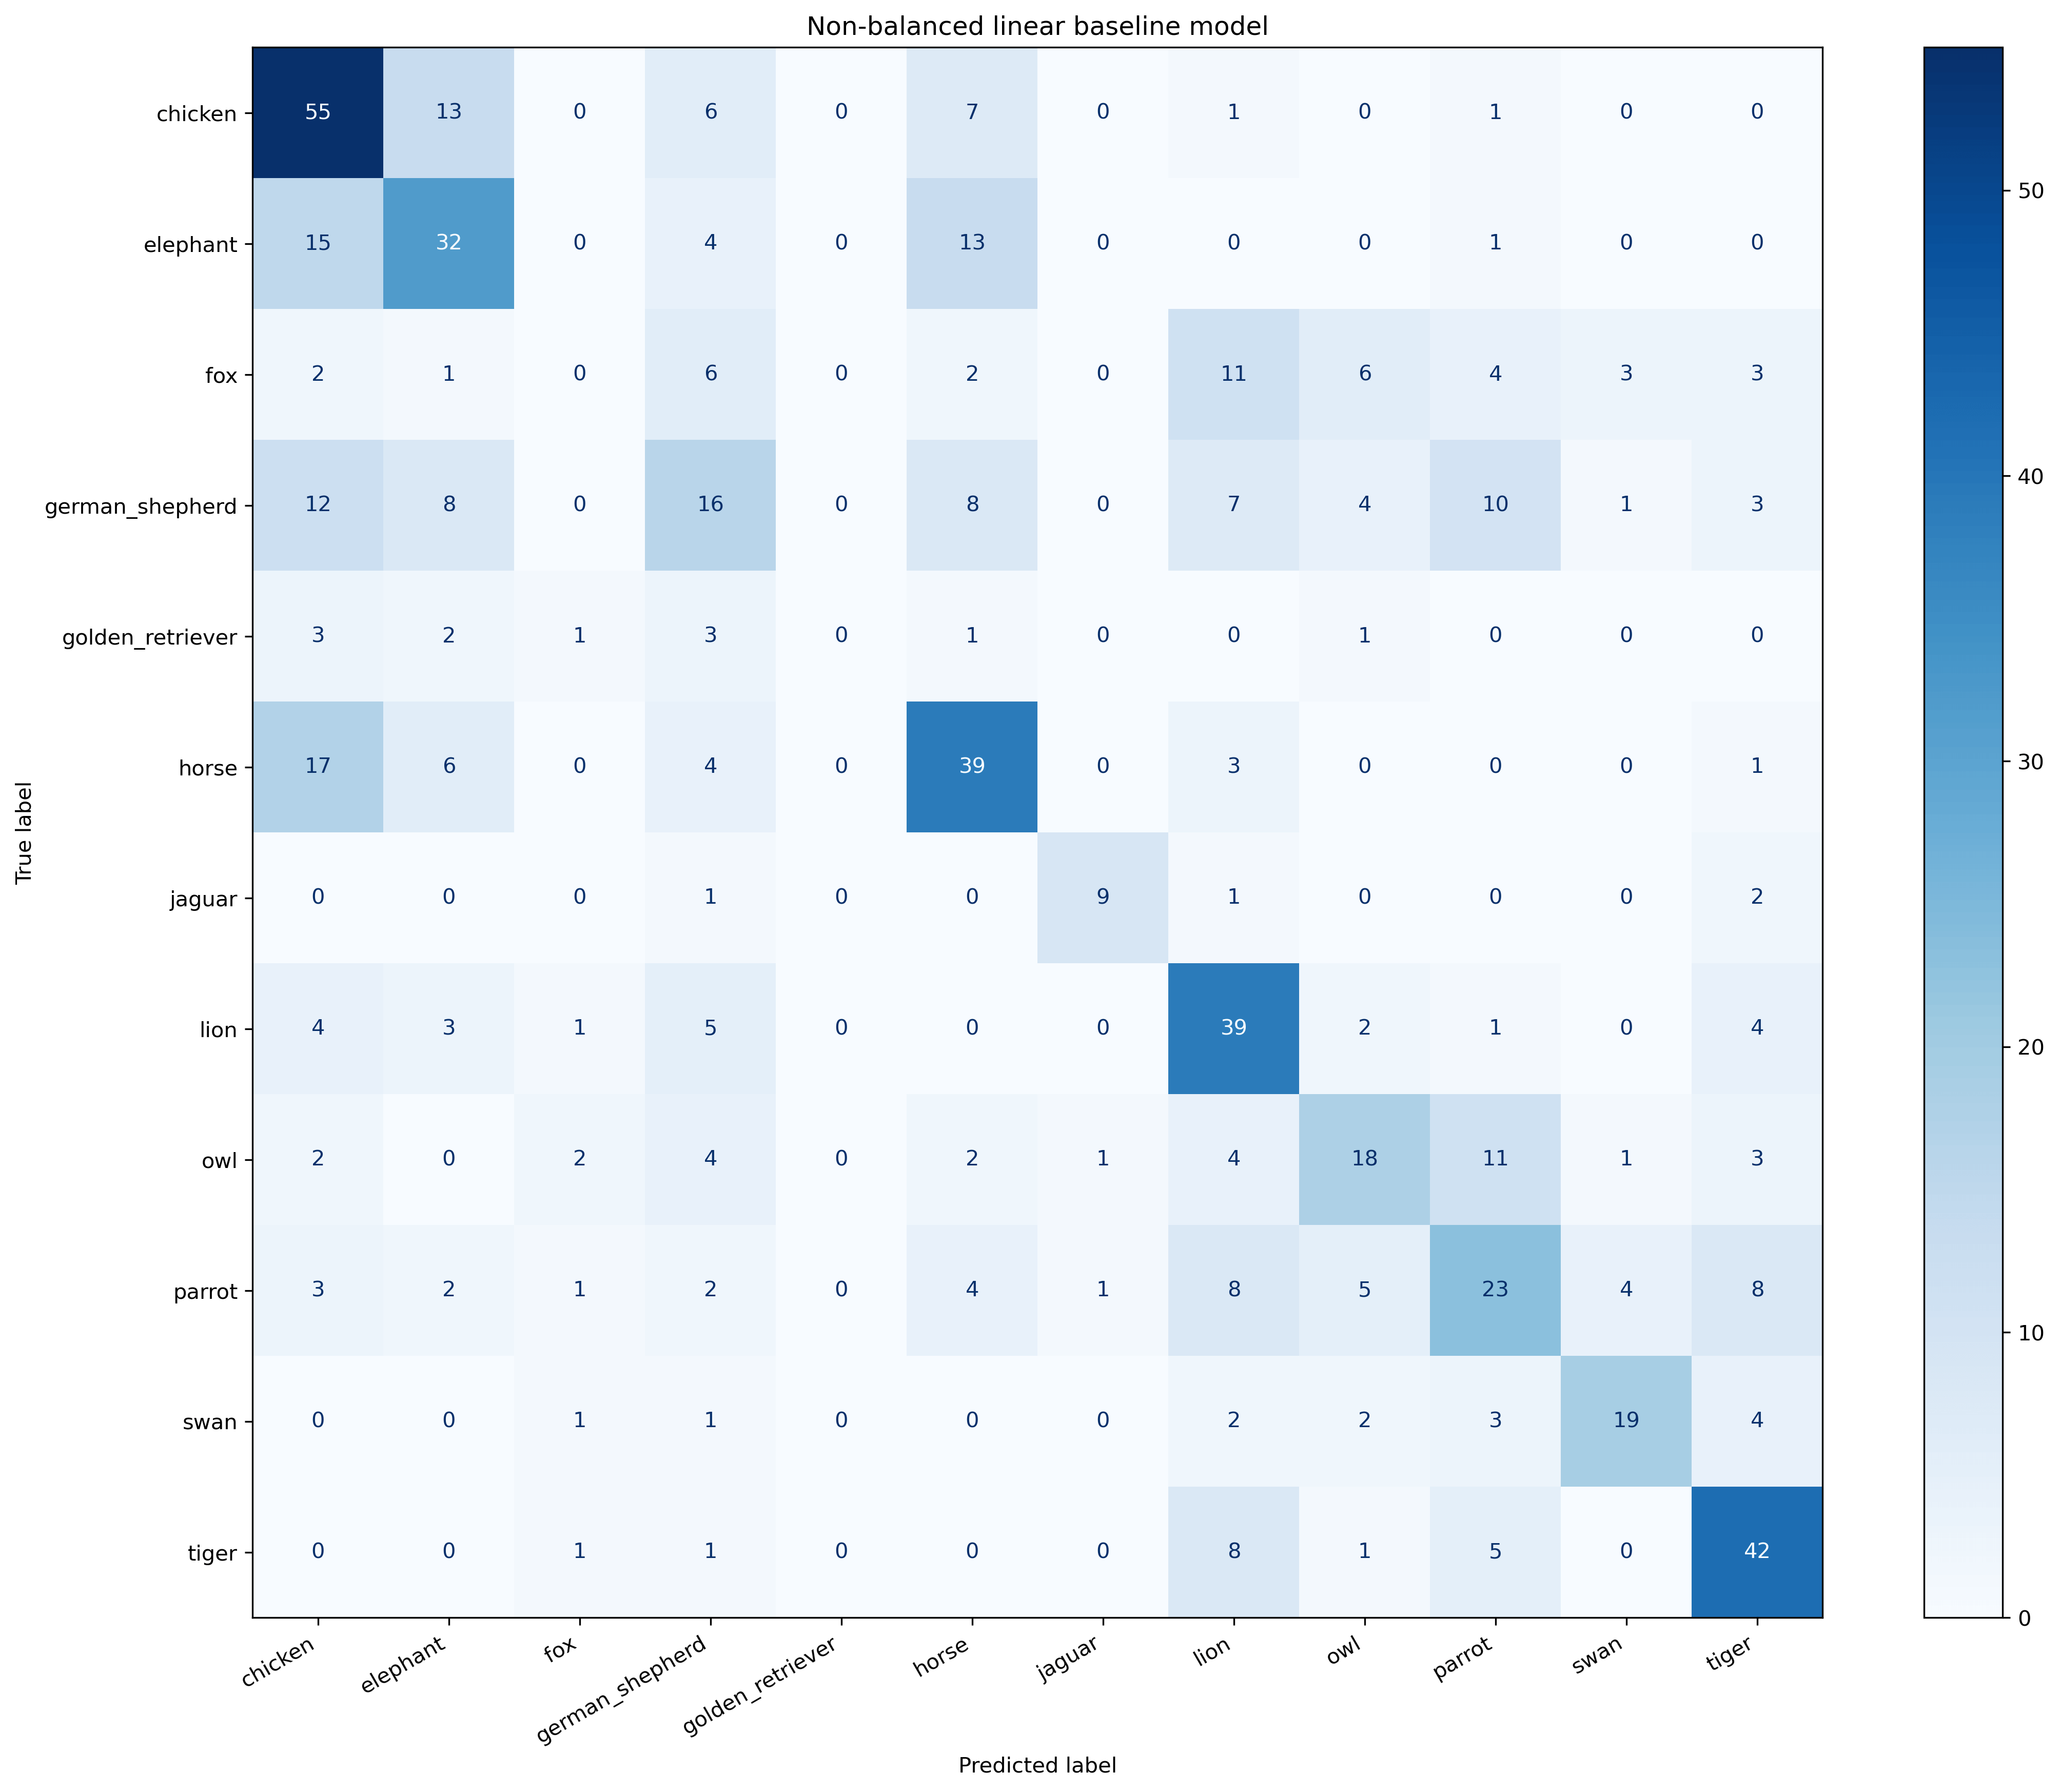
\includegraphics[width=\textwidth]{images/MA/MA_LBM_non_normalised.png}}
        \captionsetup{width=0.9\linewidth}
        \captionsetup{justification=centering}
        \caption{Non normalised CM.}
    \end{subfigure}
    \hspace{1cm}
    \begin{subfigure}{.45\textwidth}
        \centering
        \fbox{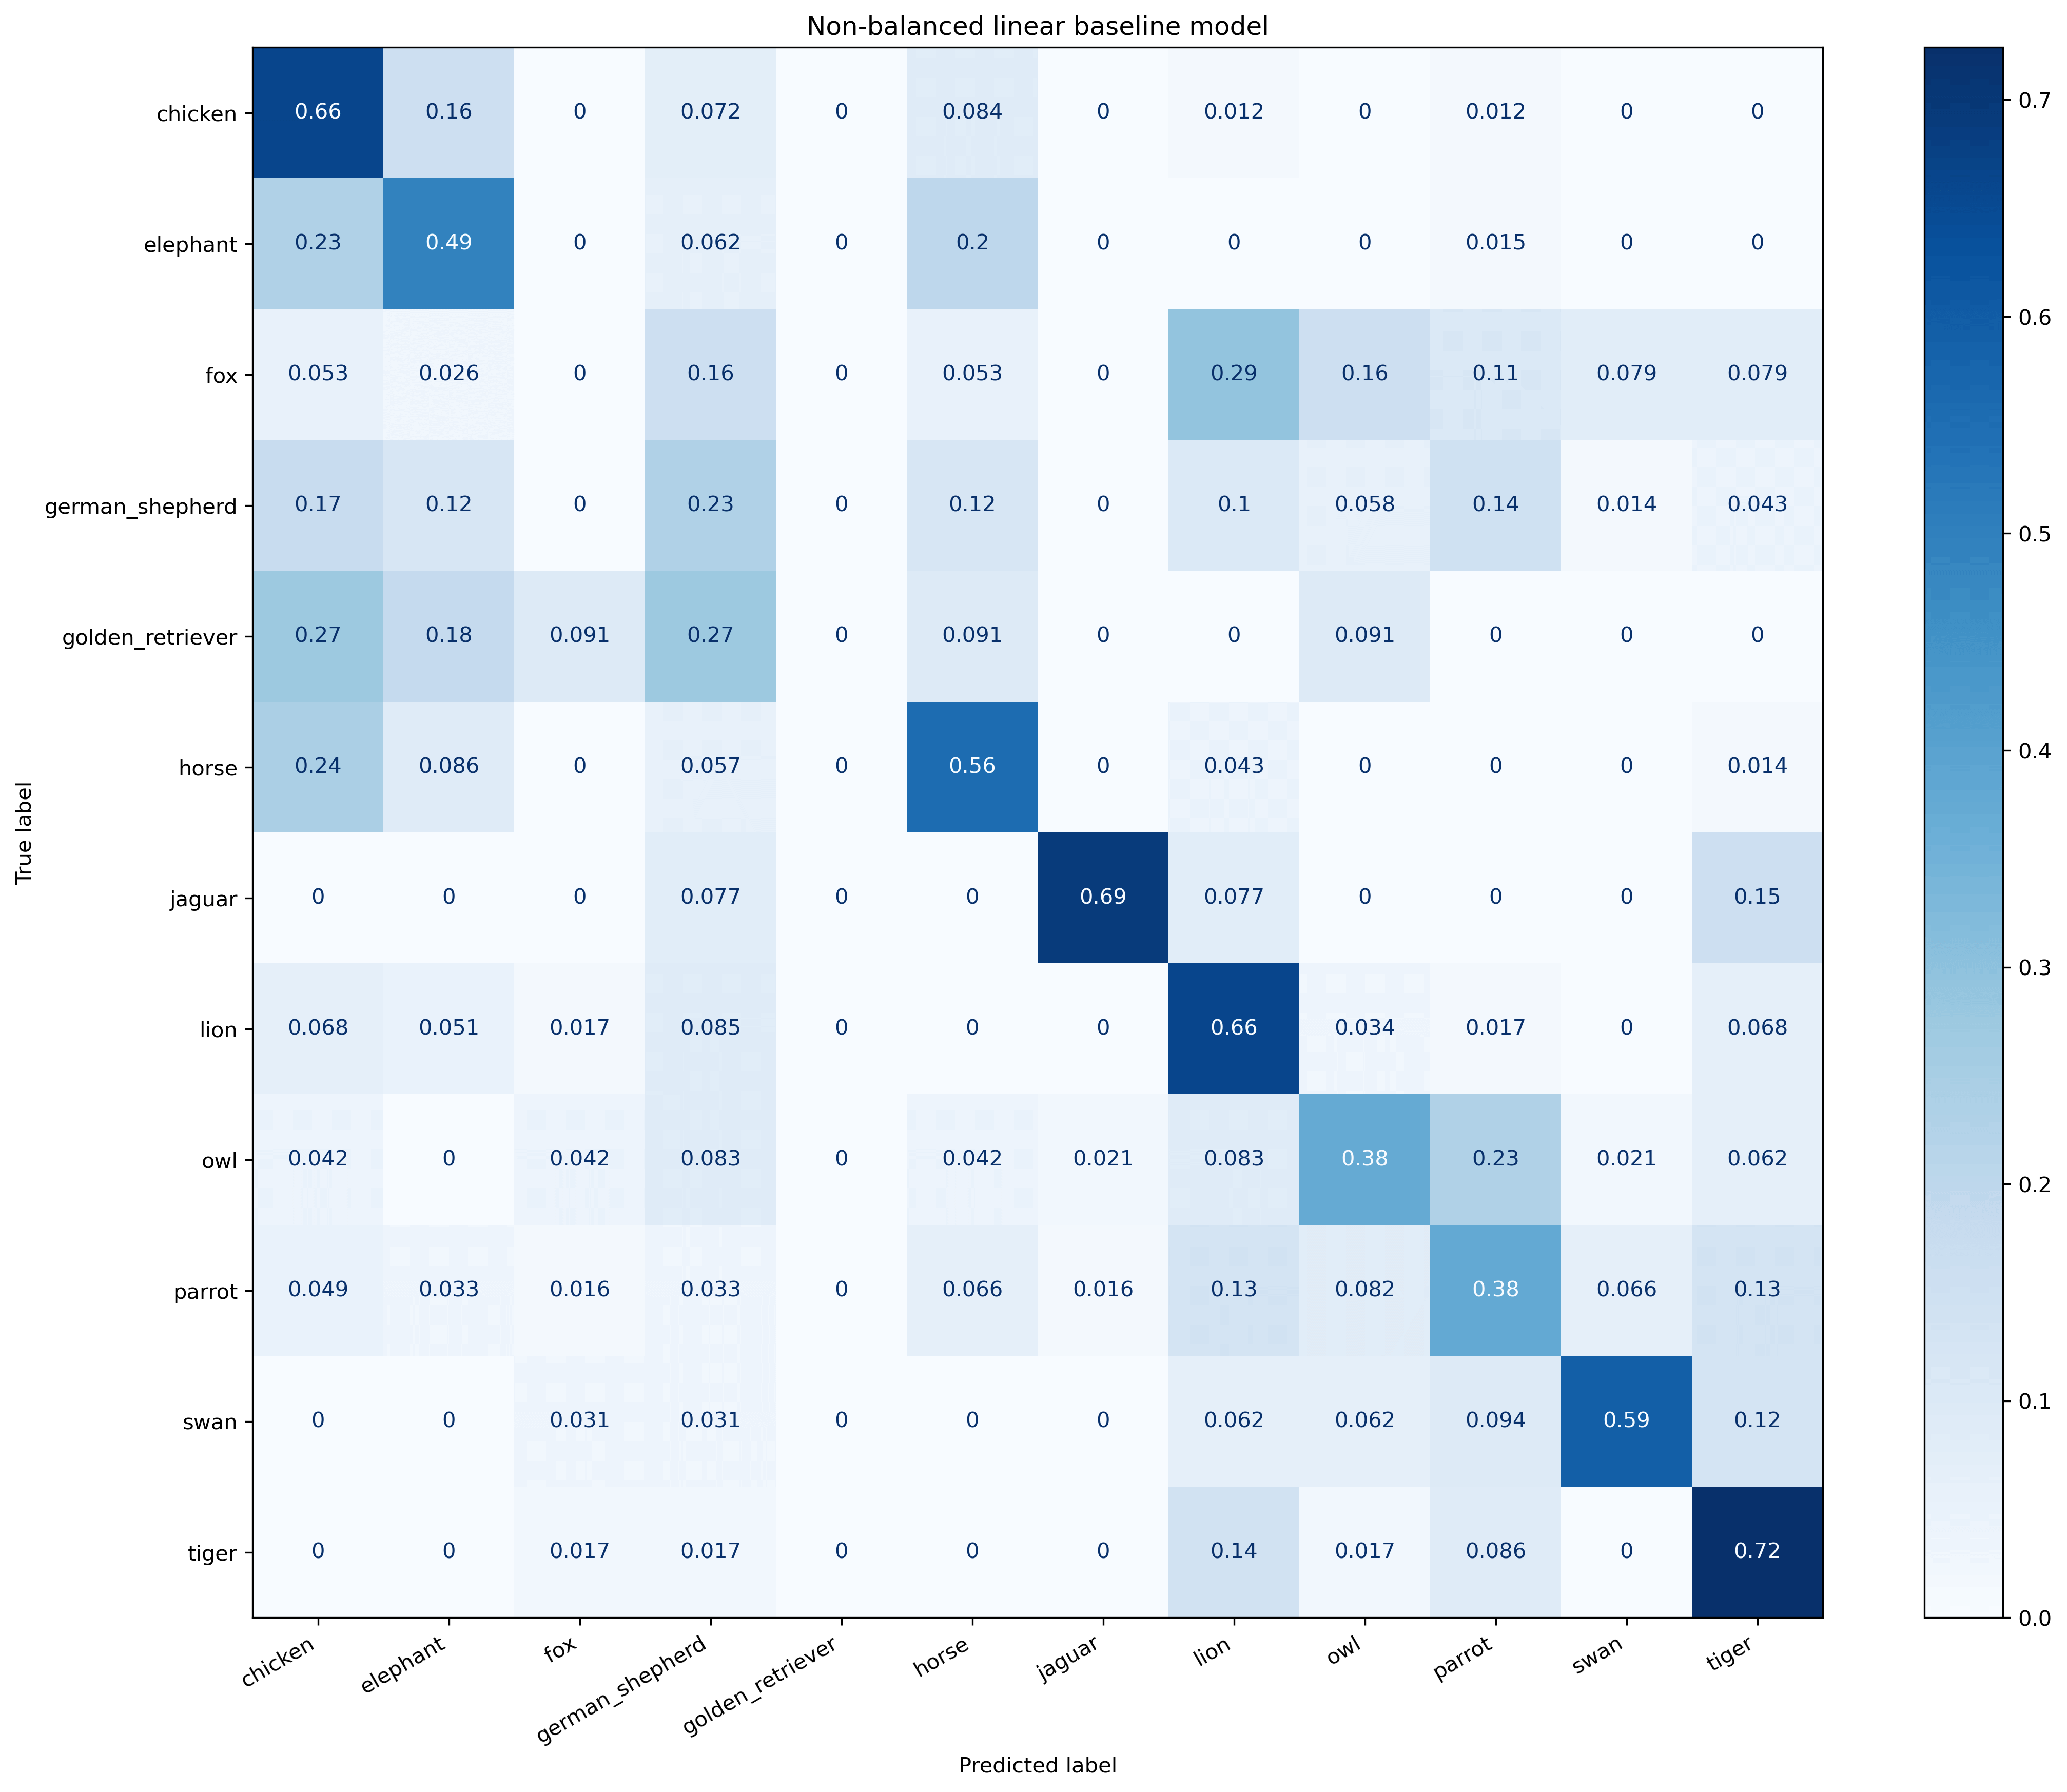
\includegraphics[width=\textwidth]{images/MA/MA_LBM_normalised.png}}
        \captionsetup{width=0.9\linewidth}
        \captionsetup{justification=centering}
        \caption{Normalised CM.}
    \end{subfigure}
    \captionsetup{width=0.8\linewidth}
    \captionsetup{justification=centering}
    \caption{Confusion matrices for the non-balanced linear baseline model.}
    \label{fig:ma_lbm_cm}
\end{figure*}

%------------------------------------

\section{Balanced linear baseline model}
\label{section:ma_lbm_balanced}

It was said in section \ref{section:LBM_finetuning_model} that it was weird the balanced LBM model received a worse MCLL score.
The confusion matrices given in figure \ref{fig:ma_lbm_cm_bal} shows a different story and teaches us multiple things, the most important of which are listed here:
\begin{itemize}
    \item The model now has some succession for each class, all be it low. This behaviour is more preferred and whilst it had a worse MCLL score it's confusion matrix shows it had a better understanding of the problem. The worse MCLL score is most likely due to the unbalance in the test set and when using CSV, the worse Kaggle score suggest the test data for the public leaderboard is also unbalanced.
    \item The correct classification of most classes has risen. These few that have dropped are classes with a high frequency suggesting it's better labelling was based on frequency bias instead of conceptual understanding for the non-balanced model. 
\end{itemize}

\begin{figure*}[ht]
    \centering
    \begin{subfigure}{.45\textwidth}
        \centering
        \fbox{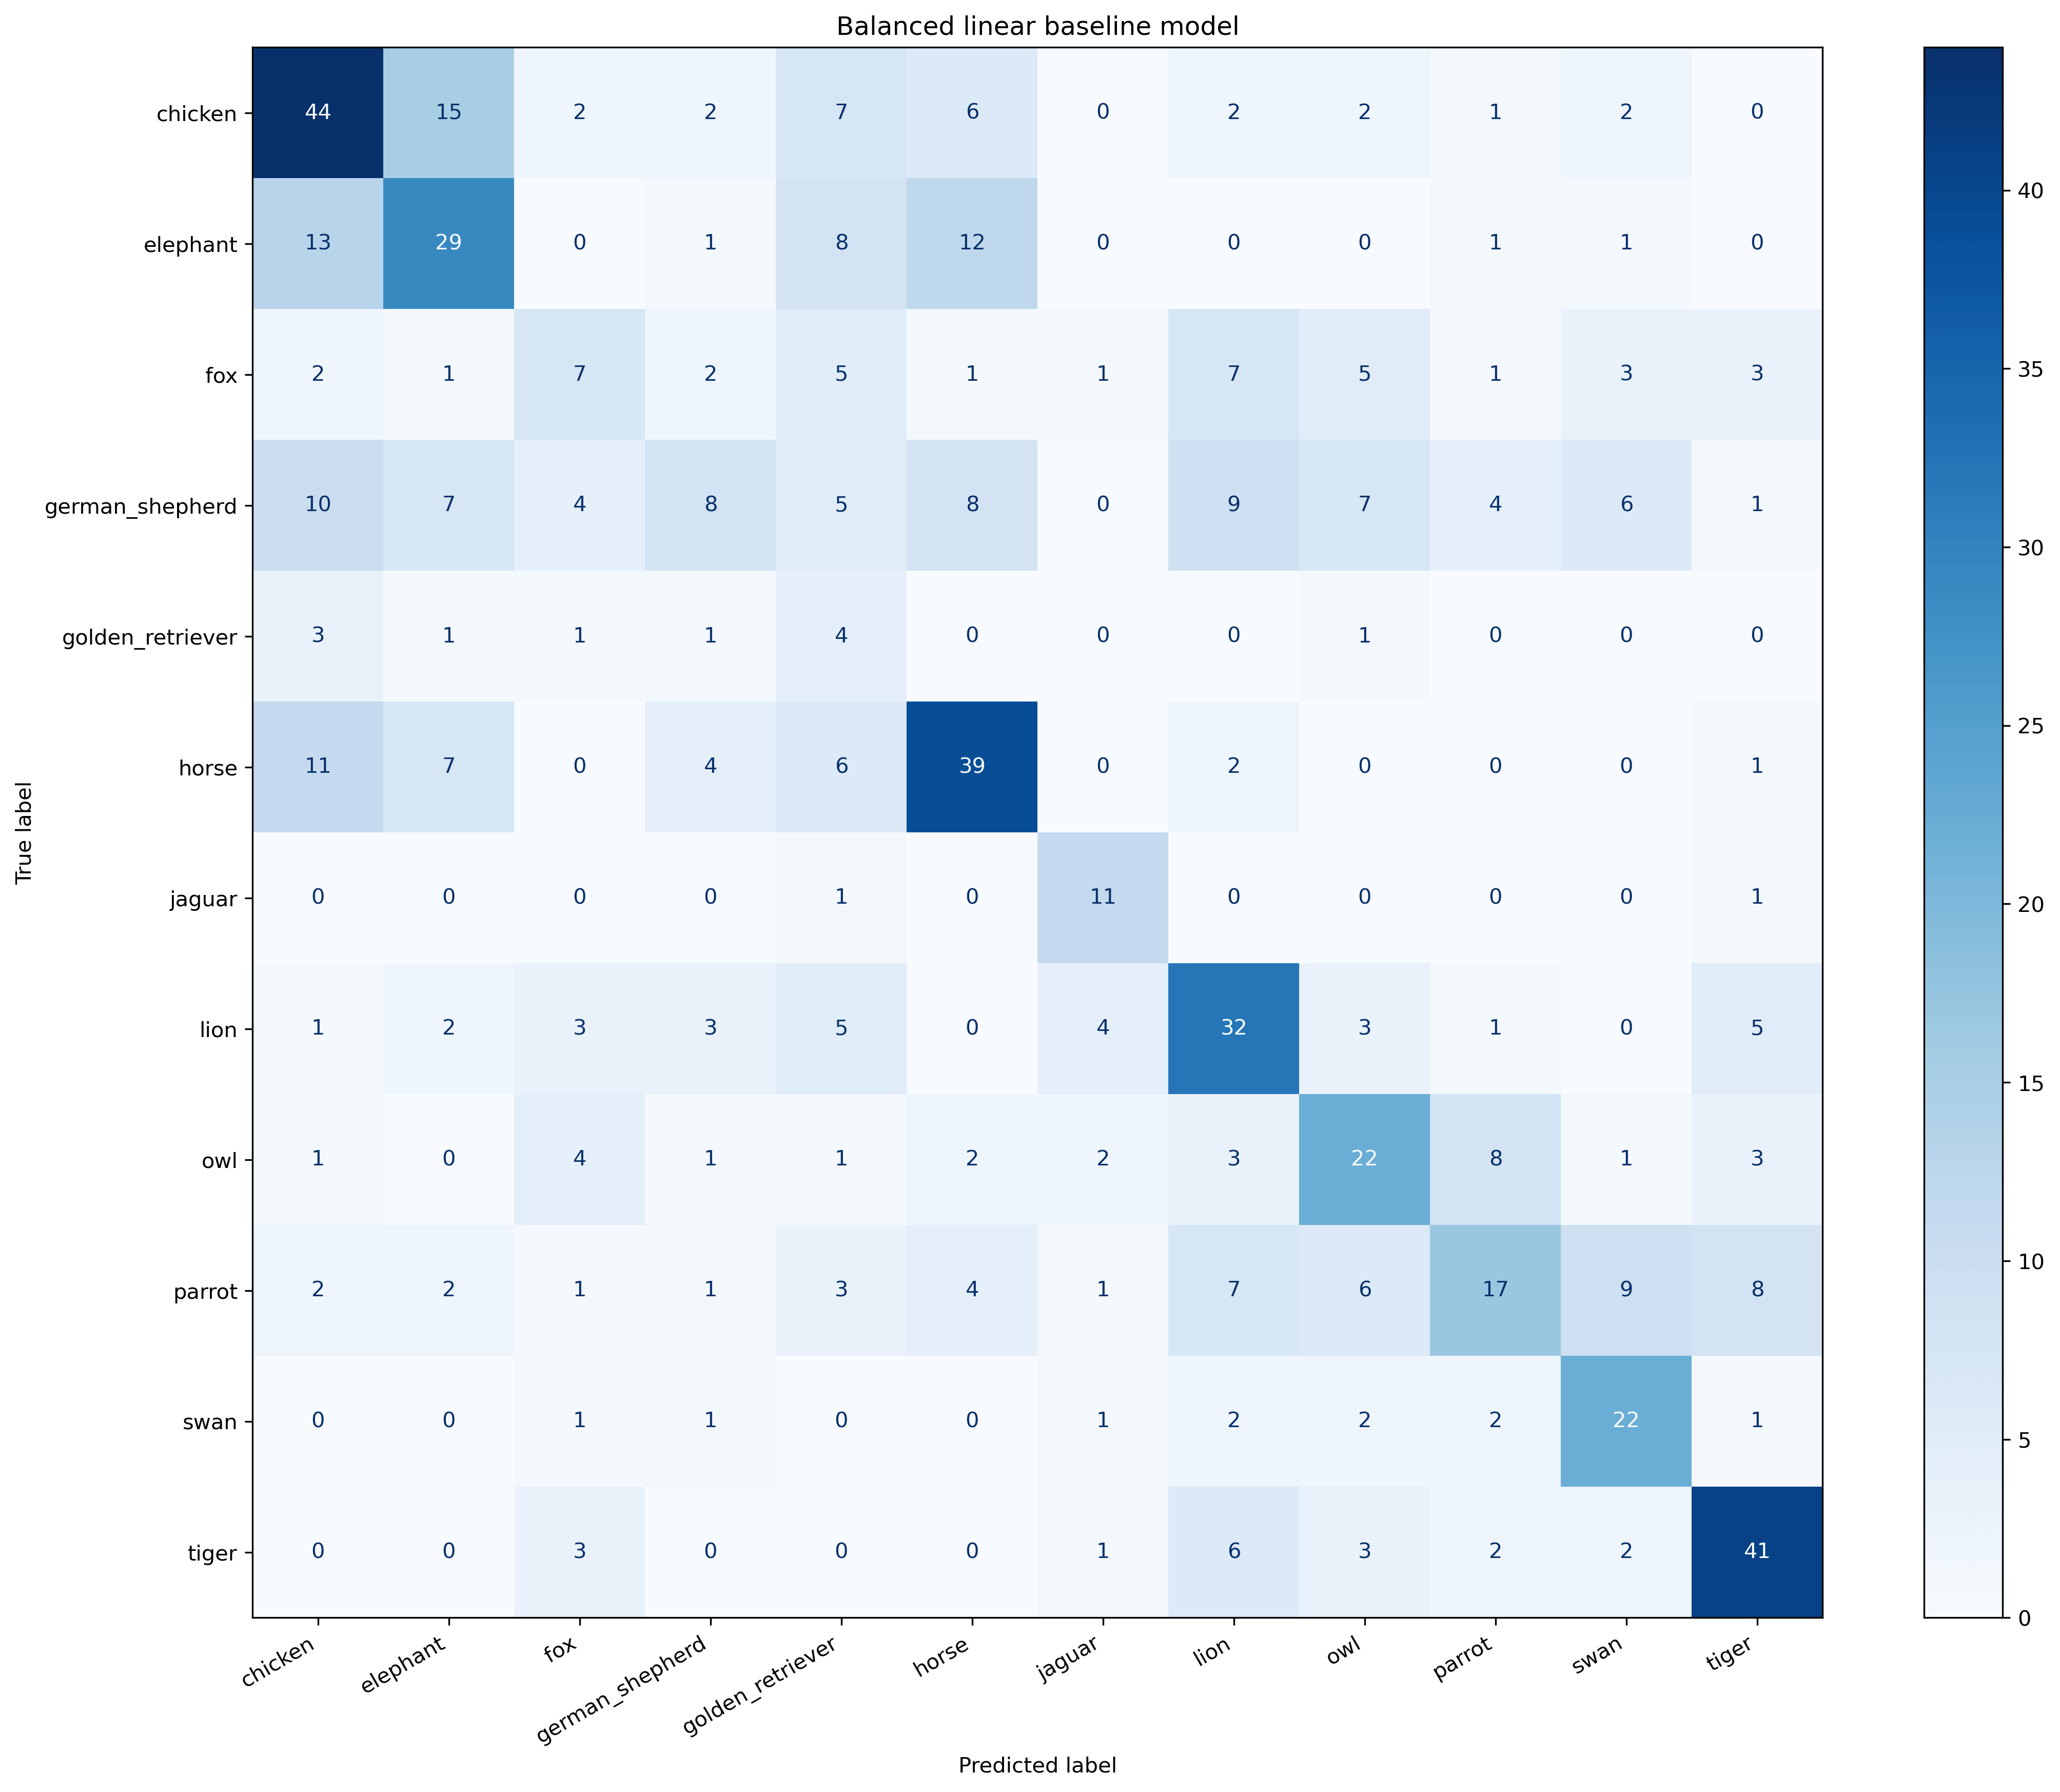
\includegraphics[width=\textwidth]{images/MA/MA_LBM_non_normalised_balanced.png}}
        \captionsetup{width=0.9\linewidth}
        \captionsetup{justification=centering}
        \caption{Non normalised CM.}
    \end{subfigure}
    \hspace{1cm}
    \begin{subfigure}{.45\textwidth}
        \centering
        \fbox{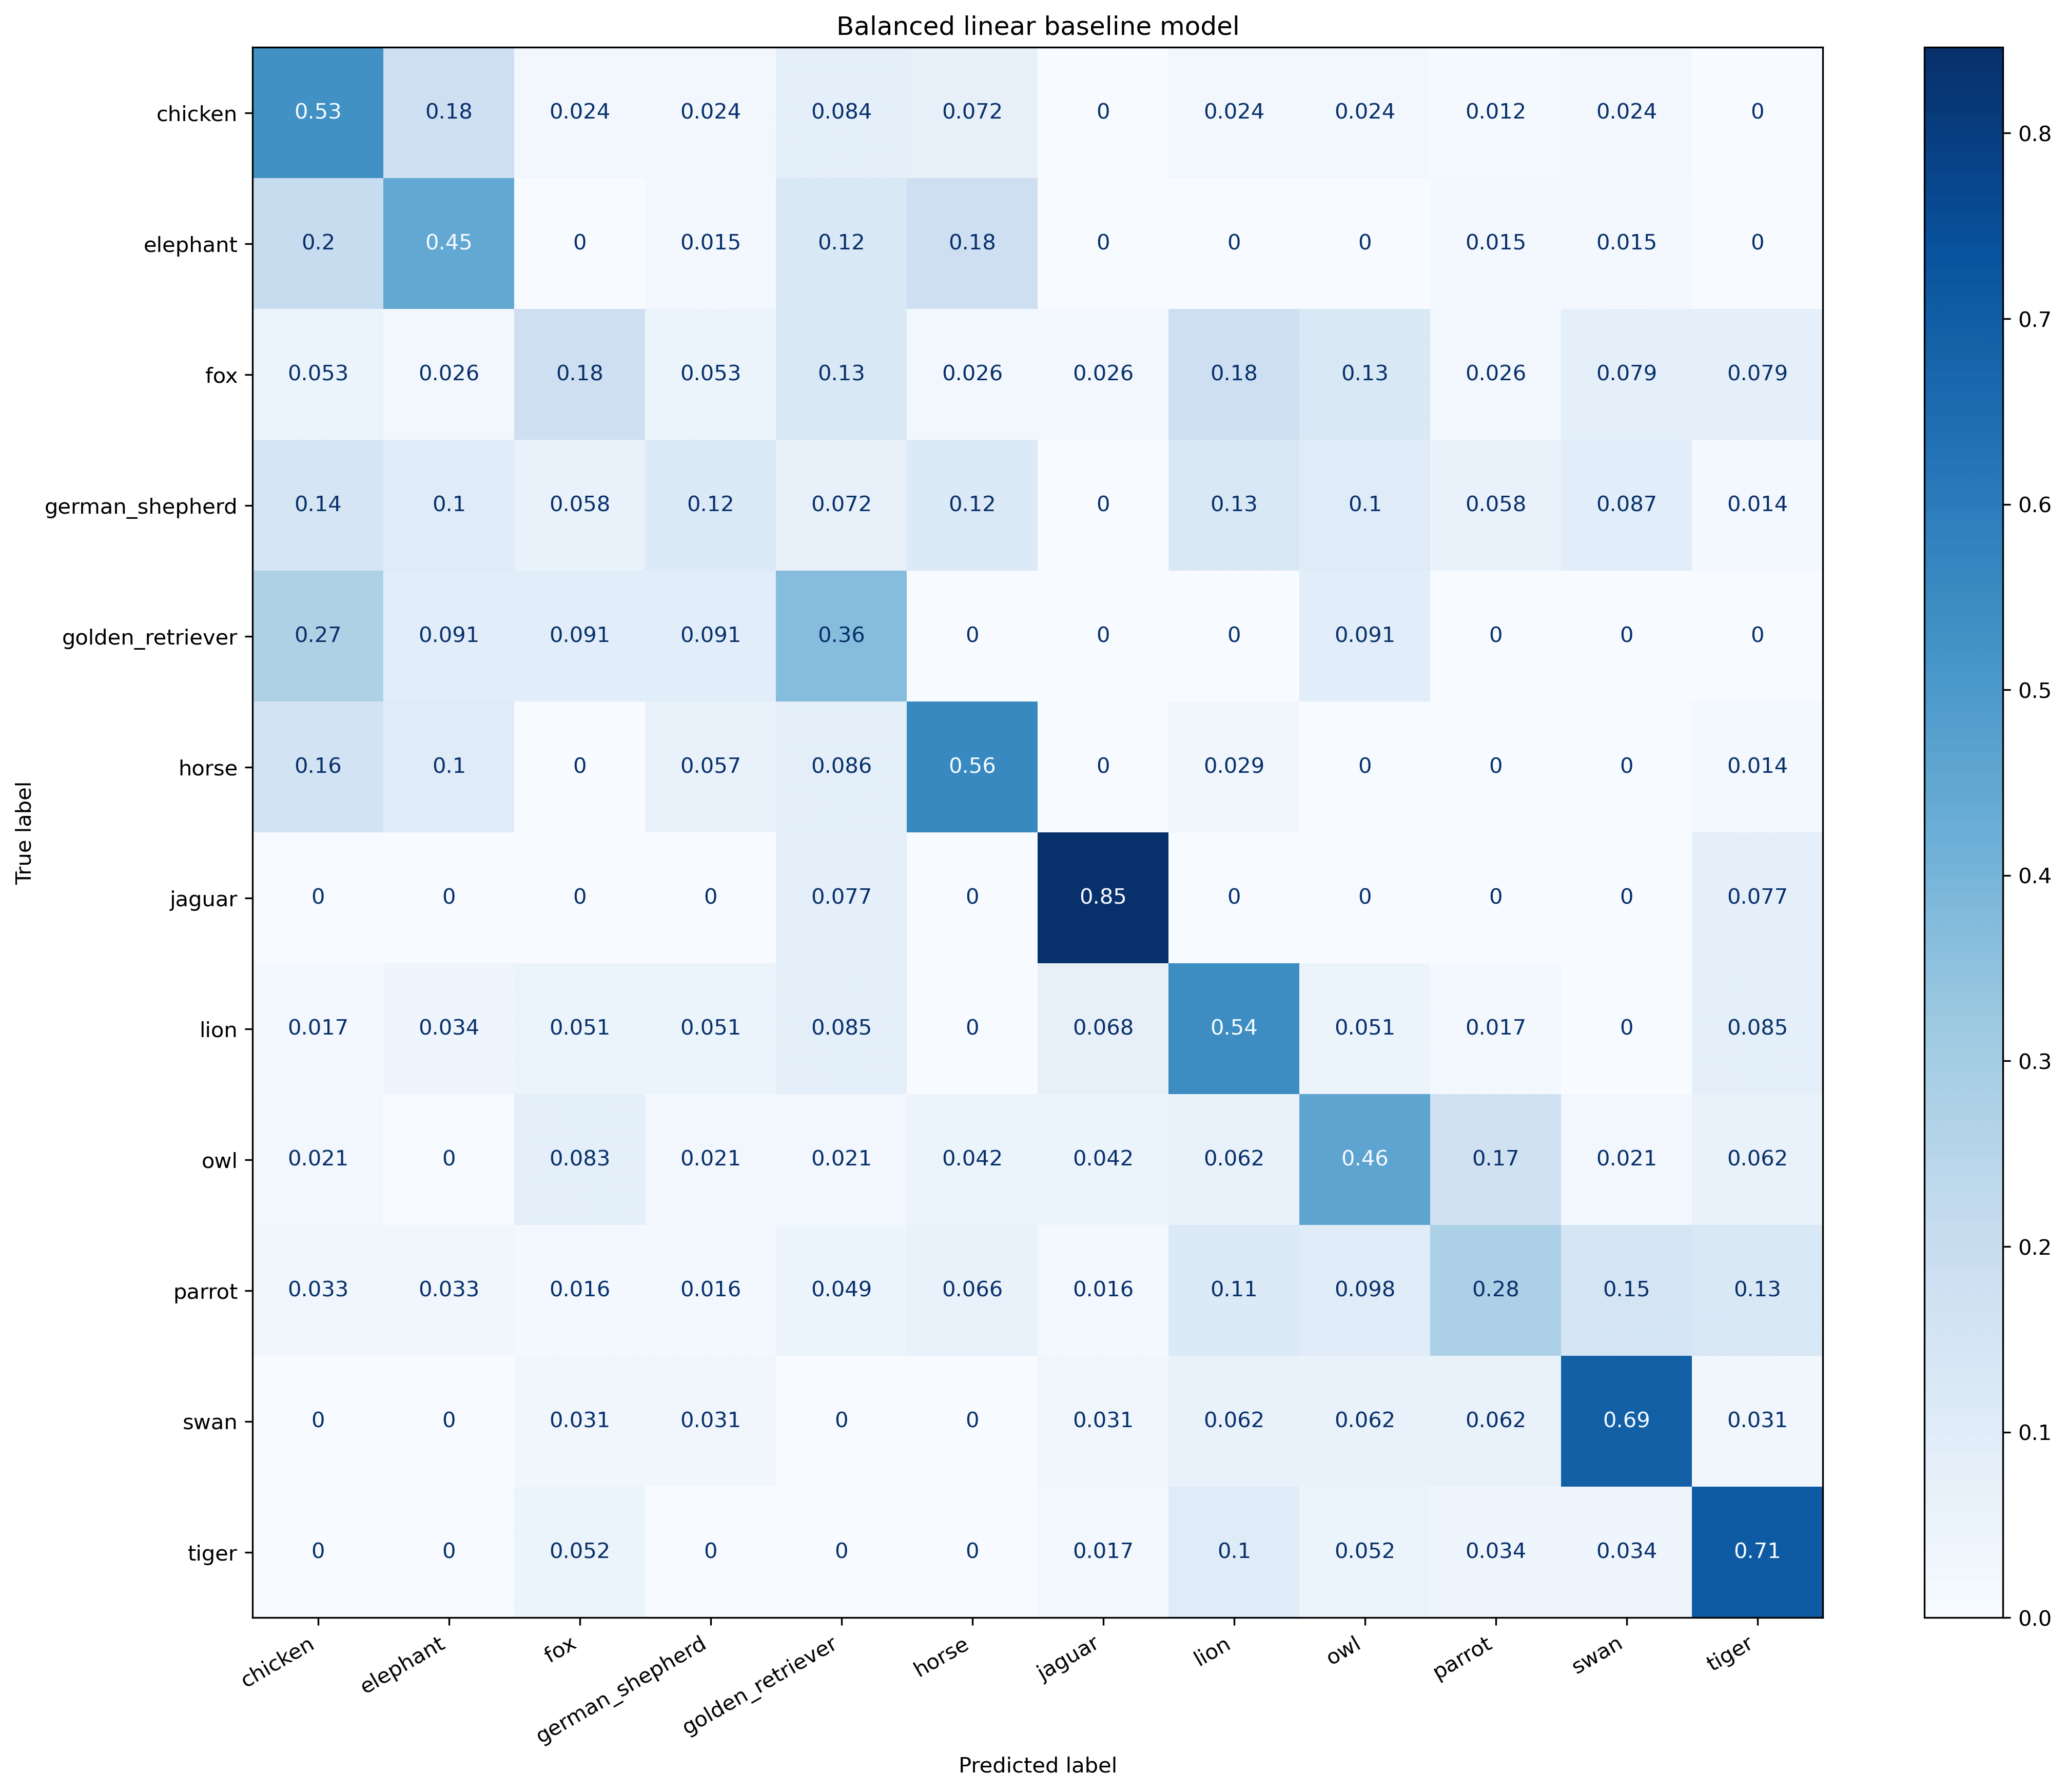
\includegraphics[width=\textwidth]{images/MA/MA_LBM_normalised_balanced.png}}
        \captionsetup{width=0.9\linewidth}
        \captionsetup{justification=centering}
        \caption{Normalised CM.}
    \end{subfigure}
    \captionsetup{width=0.8\linewidth}
    \captionsetup{justification=centering}
    \caption{Confusion matrices for the balanced linear baseline model.}
    \label{fig:ma_lbm_cm_bal}
\end{figure*}

%------------------------------------

\section{Support Vector Classifier model}
\label{section:ma_svc_balanced}

The Support Vector Classifier model was the best performing model.
This is shown in figure \ref{fig:ma_svc_cm} where the correct classification is considerably better than with the LBM. There are some important notes to be made:
\begin{itemize}
    \item The model is considerably worse at identifying golden retrievers and swans compared to the balanced LBM.
    \item The model outperforms the non-balanced LBM for almost all classes but classifying dogs and swans remains a difficult task.
    \item When wrongly classifying, the made error is comparable to the one for the balanced LBM, e.g. a fox is often misinterpreted as a lion. This suggests there's a correlation between these classes.
\end{itemize}

\begin{figure*}[ht]
    \centering
    \begin{subfigure}{.45\textwidth}
        \centering
        \fbox{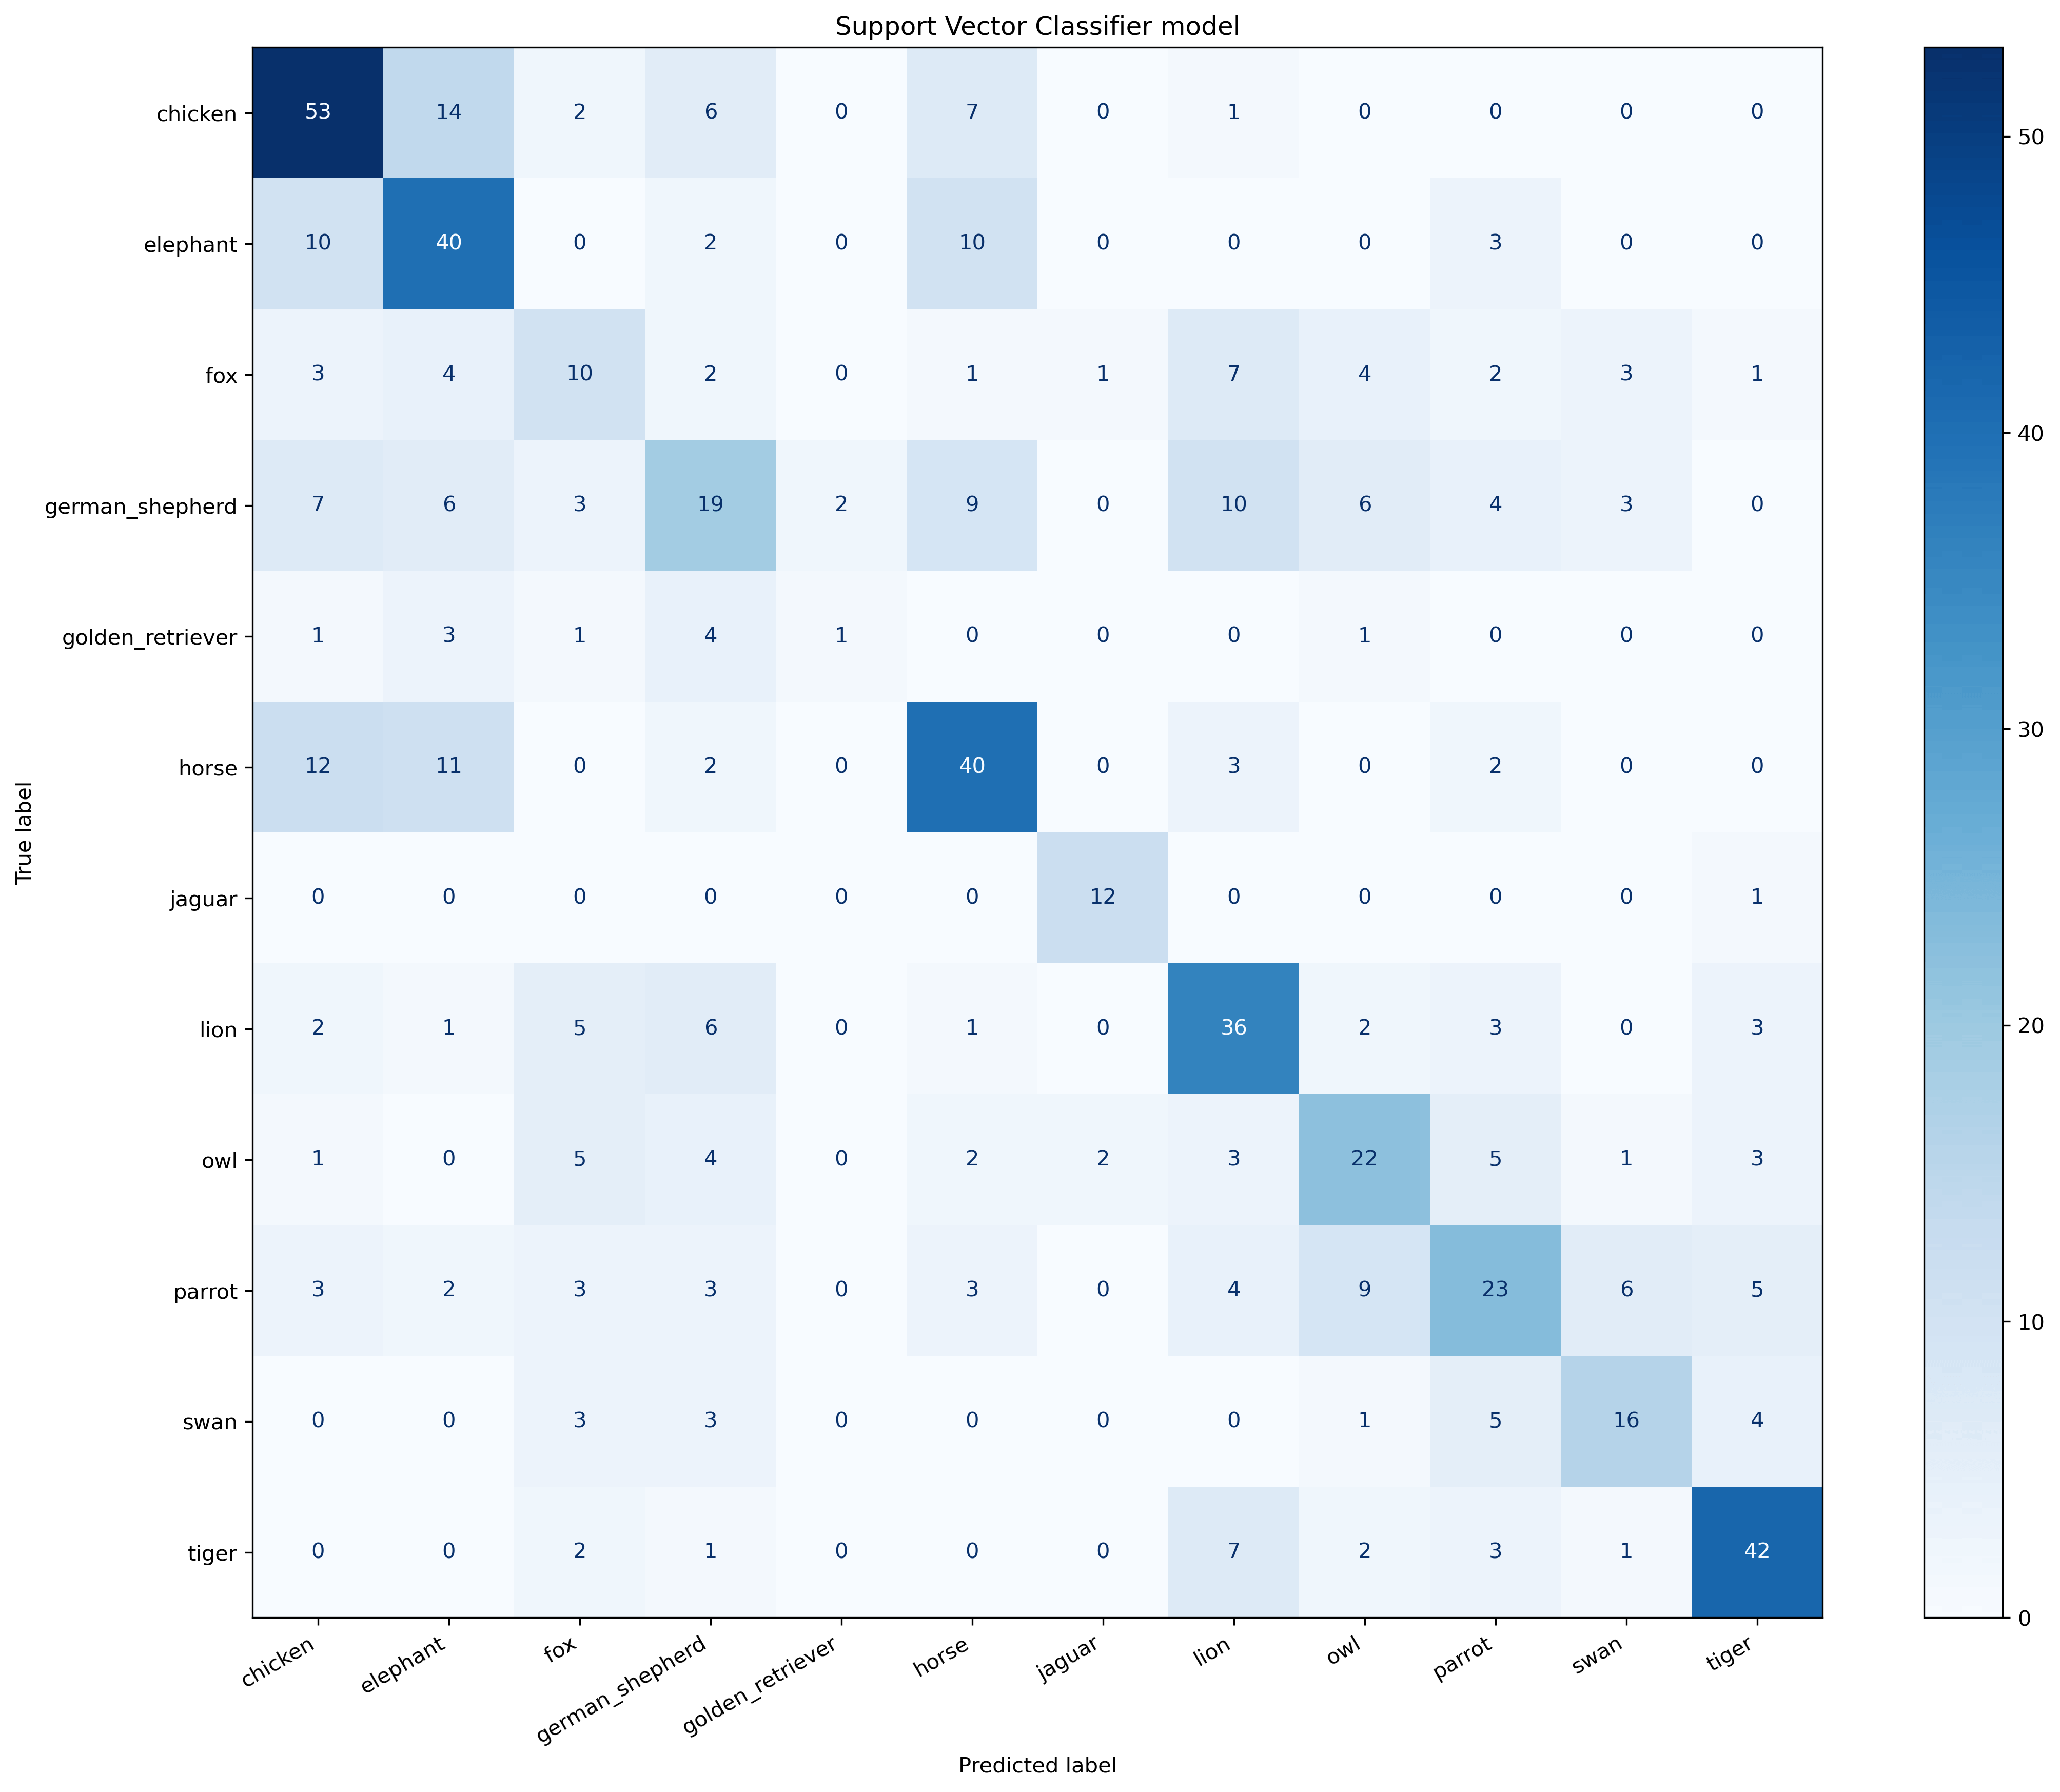
\includegraphics[width=\textwidth]{images/MA/MA_SVC_non_normalised.png}}
        \captionsetup{width=0.9\linewidth}
        \captionsetup{justification=centering}
        \caption{Non normalised CM.}
    \end{subfigure}
    \hspace{1cm}
    \begin{subfigure}{.45\textwidth}
        \centering
        \fbox{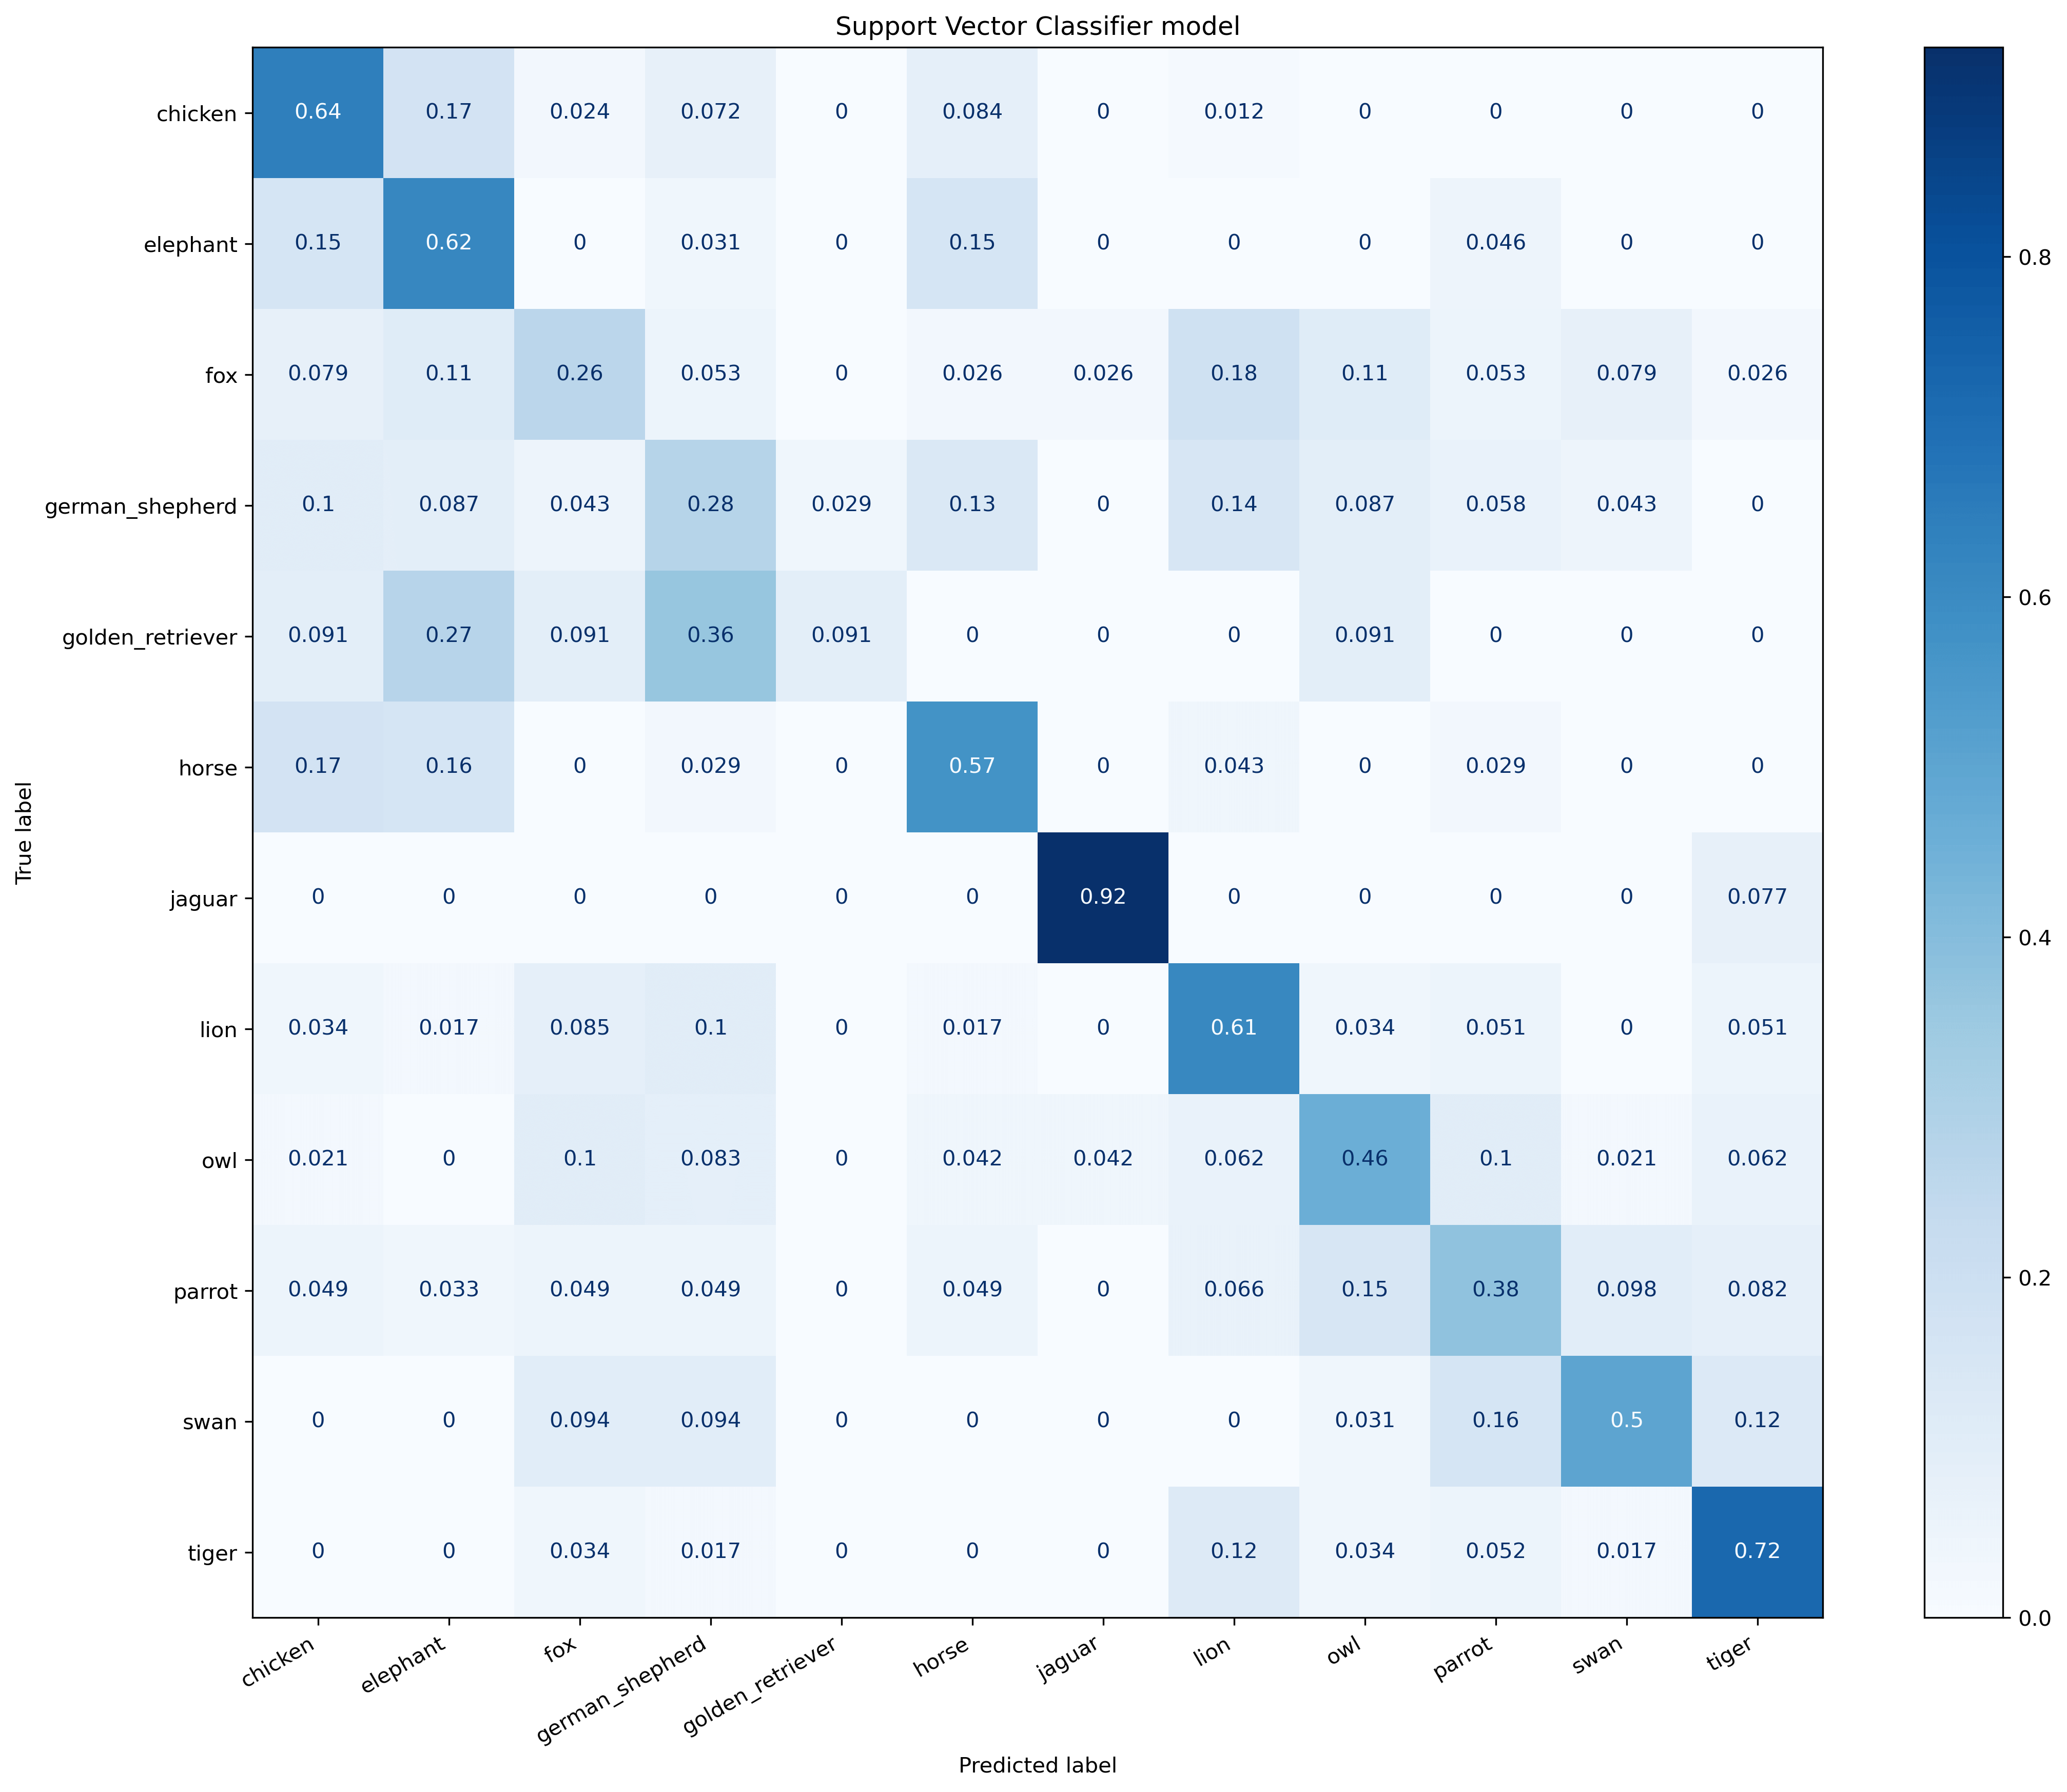
\includegraphics[width=\textwidth]{images/MA/MA_SVC_normalised.png}}
        \captionsetup{width=0.9\linewidth}
        \captionsetup{justification=centering}
        \caption{Normalised CM.}
    \end{subfigure}
    \captionsetup{width=0.8\linewidth}
    \captionsetup{justification=centering}
    \caption{Confusion matrices for the Support Vector Classifier model.}
    \label{fig:ma_svc_cm}
\end{figure*}


%------------------------------------

\section{Linear SVC and Gradient Boosting}
\label{section:ma_linSVC_grad_boost}

As discussed in part \ref{part:linear_svc}, the linear SVC variant performed worse than the just discussed SVC variant.
The confusion matrices reflect this by just performing worse overall with no noteworthy other differences.
For completeness the matrices are given in the extra's figures list (figure \ref{fig:ma_linsvc_cm}).

As discussed in part \ref{part:gradien_boost}, the Gradient Boosting model didn't perform that well.
This is also reflected in the confusion matrices, given in figure \ref{fig:ma_gb_cm}, with worse overall scores than both the SVC model and balanced LBM model.
One important thing to note is that the gradient boosting algorithm performed well on parrots compared to the other models, with an accuracy of 50\%.

\begin{figure*}[ht]
    \centering
    \begin{subfigure}{.45\textwidth}
        \centering
        \fbox{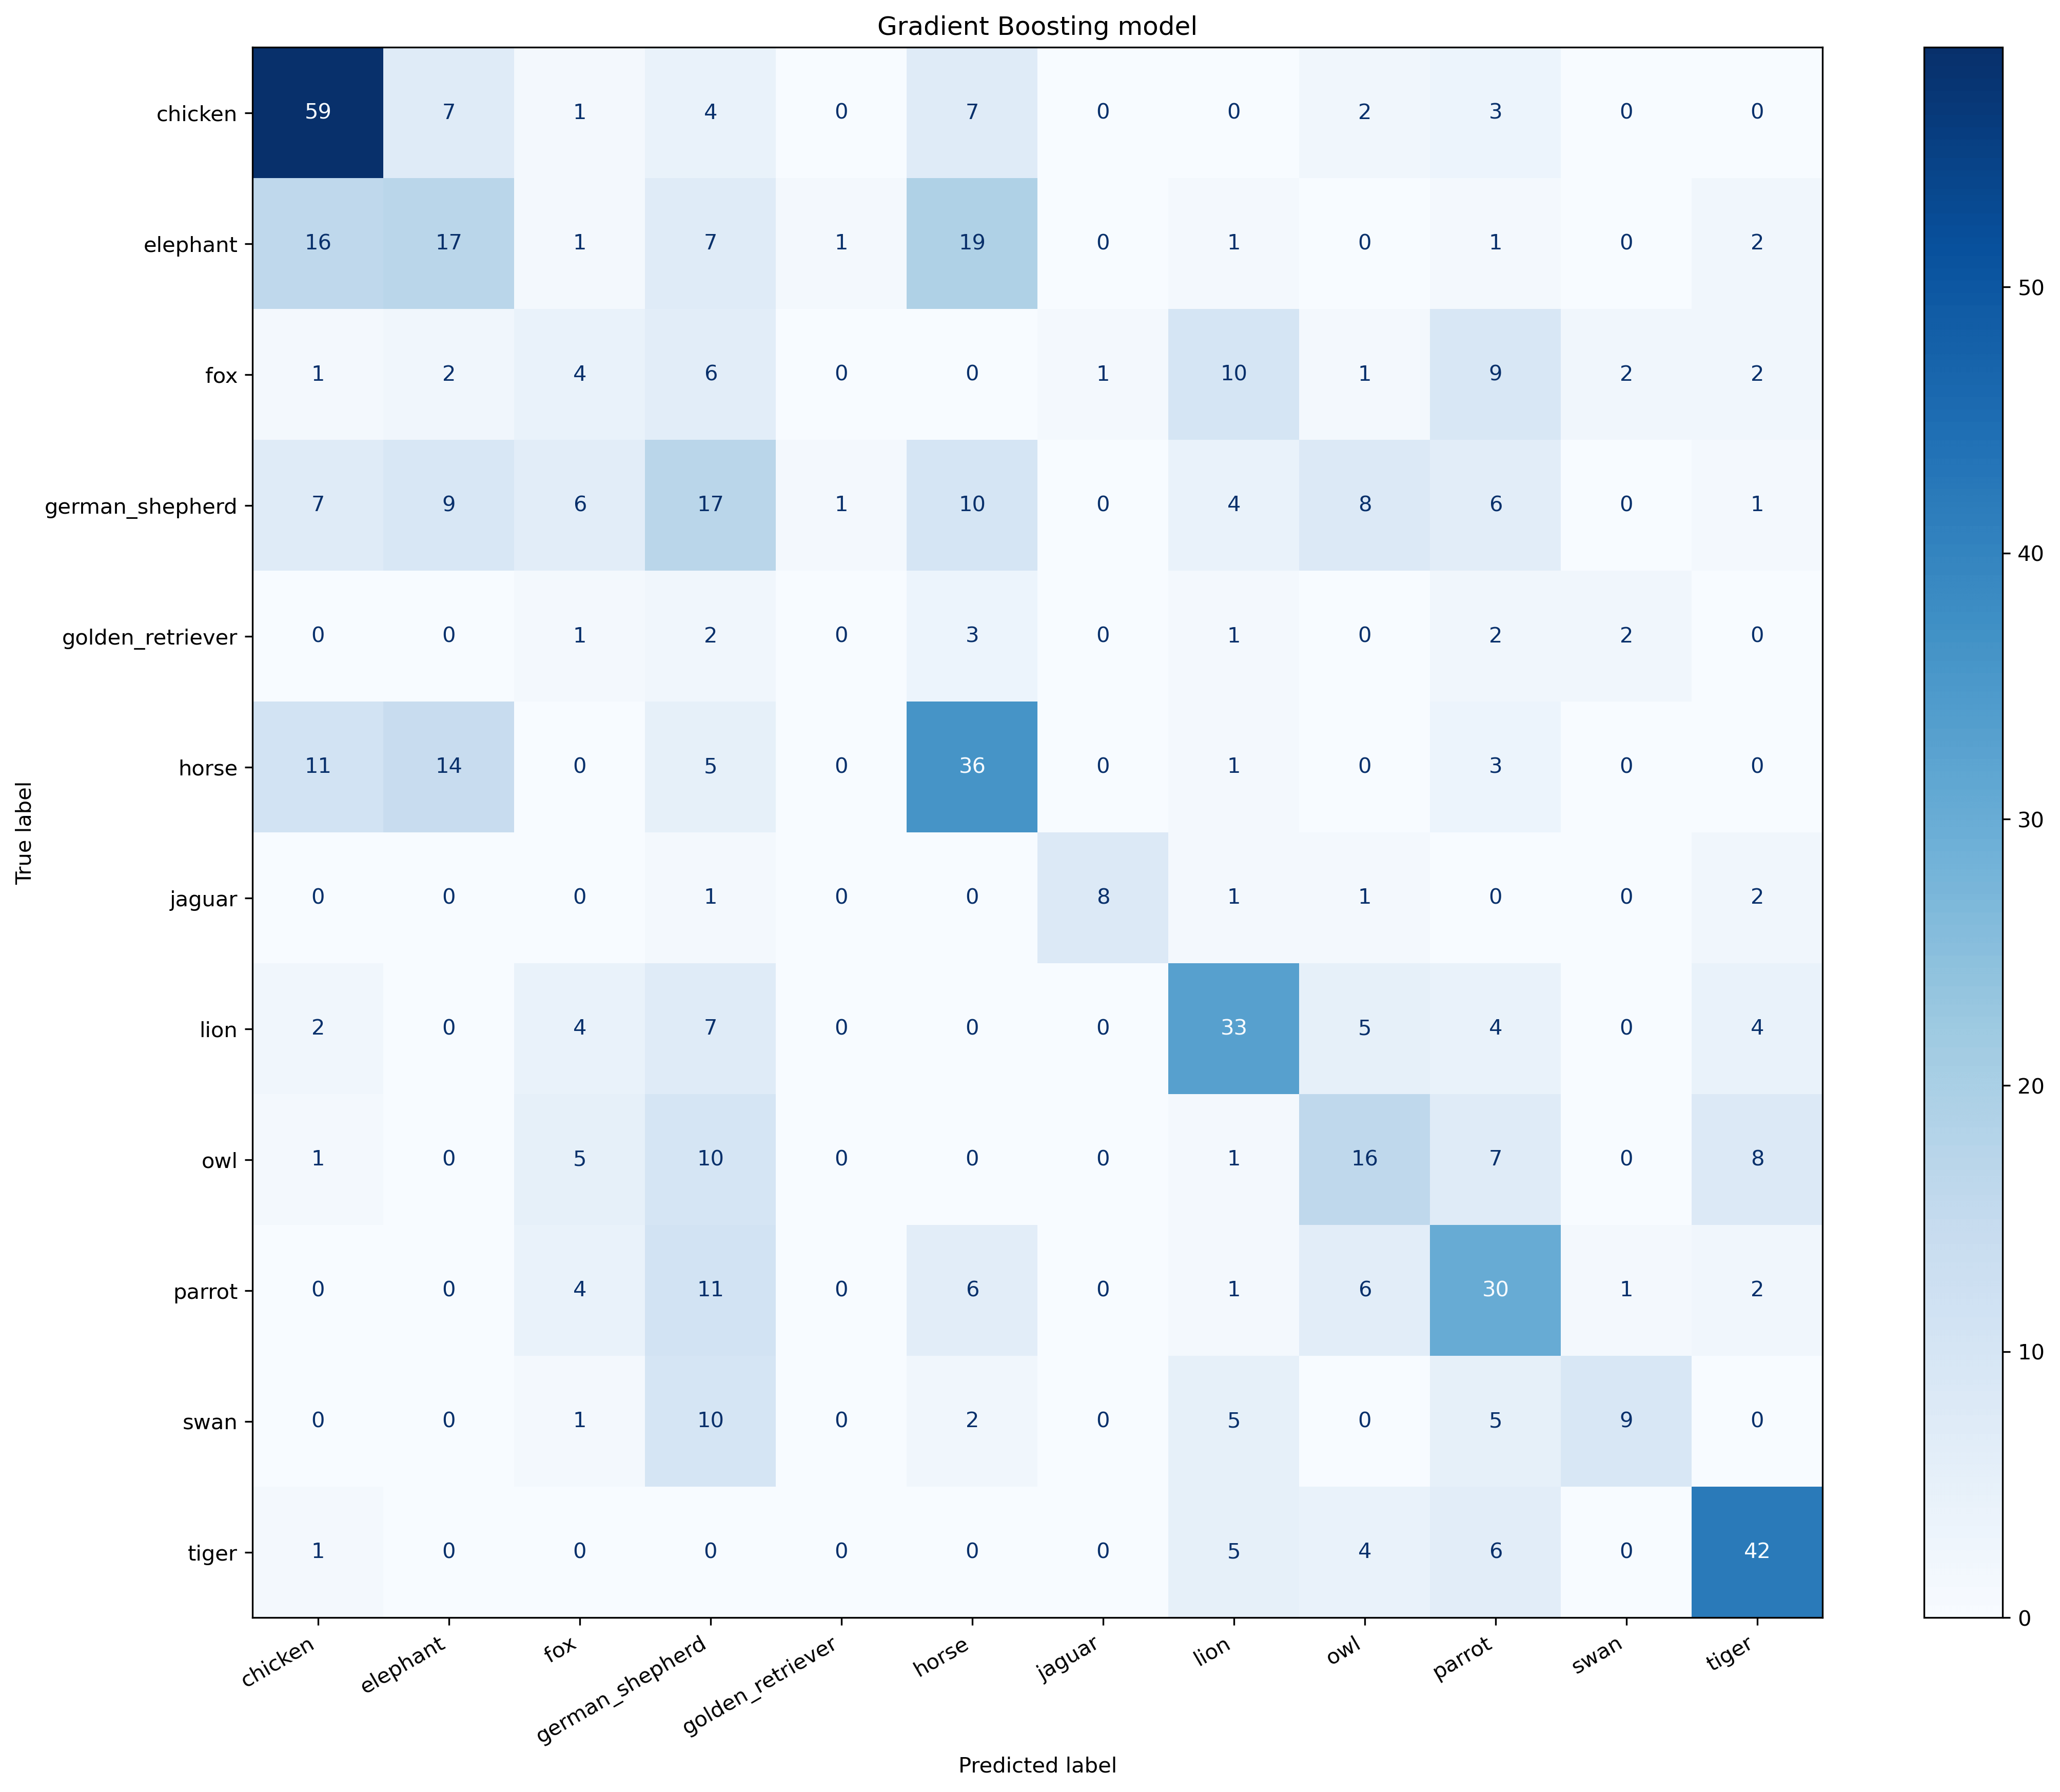
\includegraphics[width=\textwidth]{images/MA/MA_gb_non_normalised.png}}
        \captionsetup{width=0.9\linewidth}
        \captionsetup{justification=centering}
        \caption{Non normalised CM.}
    \end{subfigure}
    \hspace{1cm}
    \begin{subfigure}{.45\textwidth}
        \centering
        \fbox{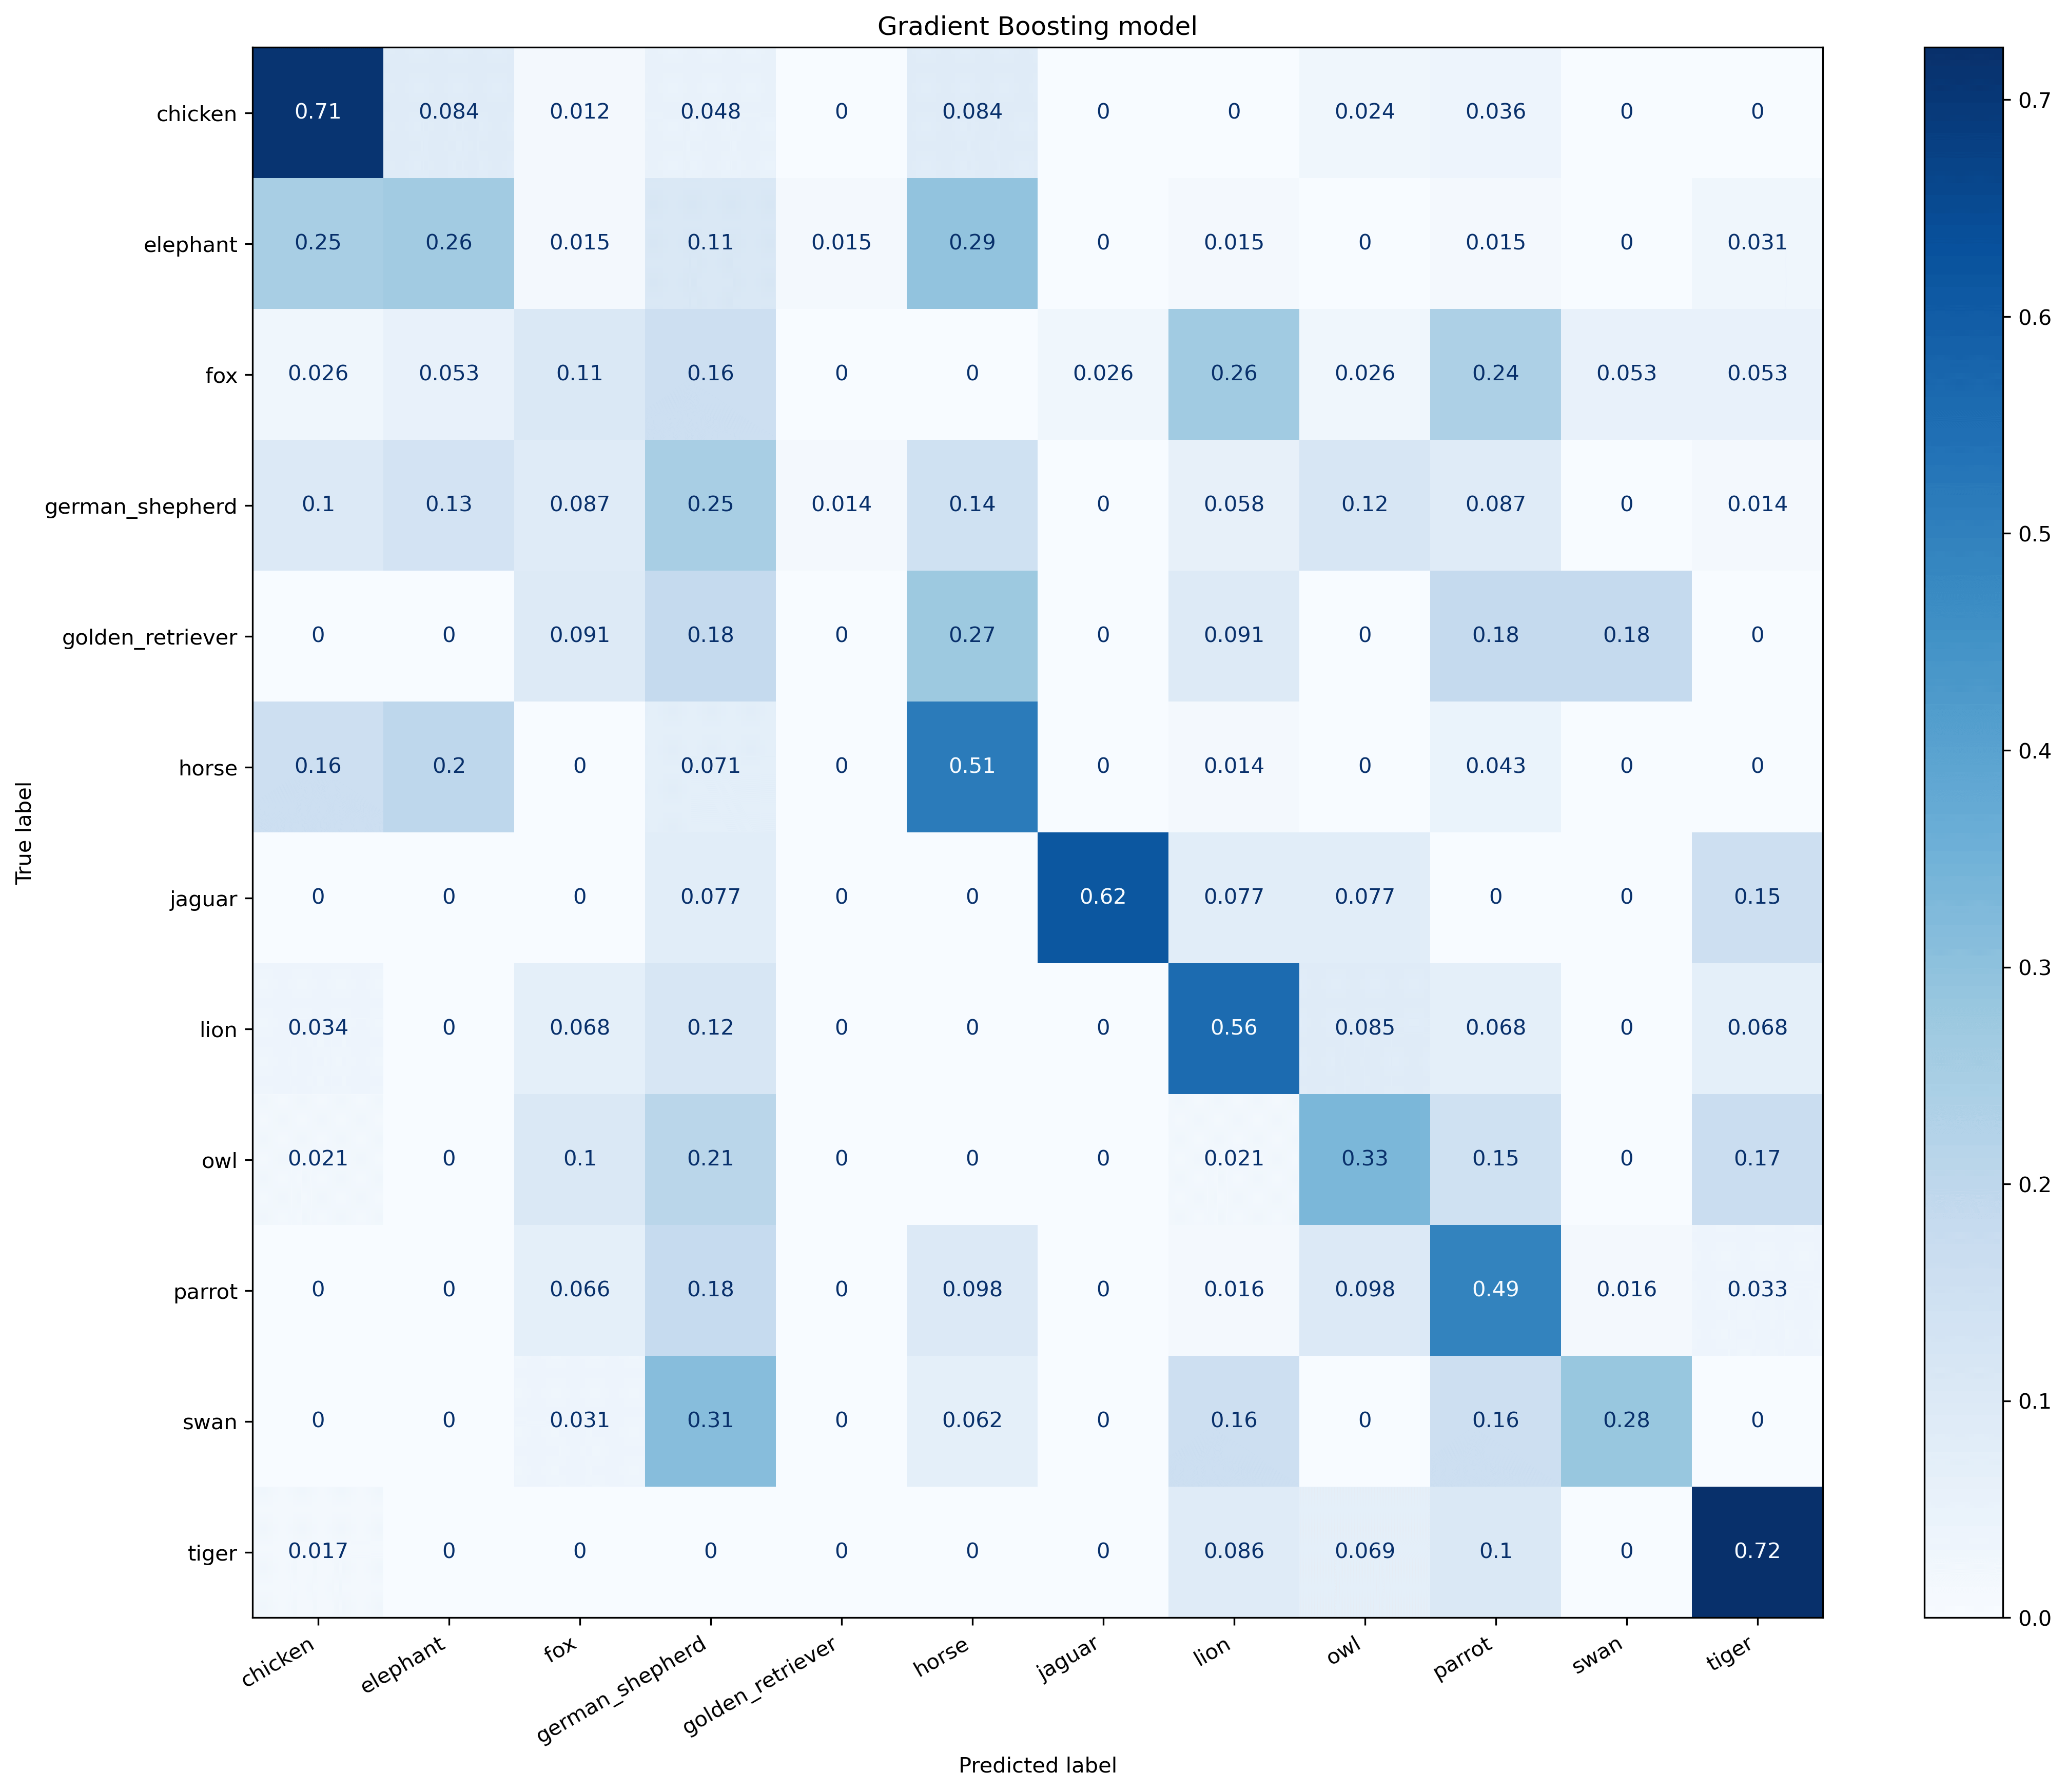
\includegraphics[width=\textwidth]{images/MA/MA_gb_normalised.png}}
        \captionsetup{width=0.9\linewidth}
        \captionsetup{justification=centering}
        \caption{Normalised CM.}
    \end{subfigure}
    \captionsetup{width=0.8\linewidth}
    \captionsetup{justification=centering}
    \caption{Confusion matrices for the Gradient Boosting model.}
    \label{fig:ma_gb_cm}
\end{figure*}